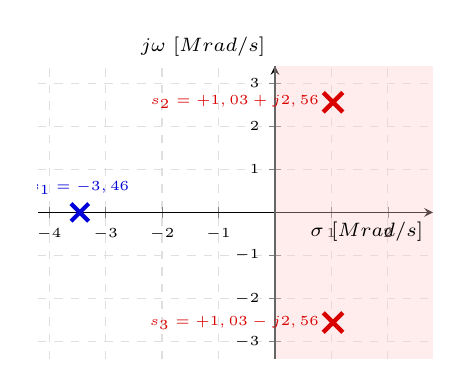
\begin{tikzpicture}
  \begin{axis}[
    width=6.6cm, height=5.3cm,
    axis lines=middle,
    xlabel={$\sigma$ [$\text{Mrad/s}$]},
    ylabel={$j\omega$ [$\text{Mrad/s}$]},
    xlabel style={at={(ticklabel* cs:1)}, anchor=north east, font=\scriptsize},
    ylabel style={at={(ticklabel* cs:1)}, anchor=south east, font=\scriptsize},
    xmin=-4.2, xmax=2.8, ymin=-3.4, ymax=3.4,
    xtick={-4, -3, -2, -1, 0, 1, 2},
    ytick={-3, -2, -1, 1, 2, 3},
    grid=both, grid style={gray!25, dashed},
    tick label style={font=\tiny},
  ]
    % Zona inestable RHP sombreada
    \fill[red!20, opacity=0.35] (axis cs:0,-3.4) rectangle (axis cs:2.8,3.4);

    % Eje jw (frontera)
    \draw[line width=1.0pt, black!60] (axis cs:0,-3.4) -- (axis cs:0,3.4);

    % Polo real LHP
    \addplot[only marks, mark=x, mark size=4.5pt, line width=1.5pt, blue!85!black]
      coordinates {(-3.455, 0)};
    \node[above=3pt, blue!85!black, font=\tiny, anchor=south] at (axis cs:-3.455, 0) {$s_1 = -3,46$};

    % Polos complejos RHP (inestables)
    \addplot[only marks, mark=x, mark size=5pt, line width=1.6pt, red!85!black]
      coordinates {(1.030, 2.558) (1.030, -2.558)};
    \node[red!85!black, font=\tiny\bfseries, anchor=east] at (axis cs:0.95, 2.558) {$s_{2} = +1,03 + j2,56$};
    \node[red!85!black, font=\tiny\bfseries, anchor=east] at (axis cs:0.95, -2.558) {$s_{3} = +1,03 - j2,56$};

  \end{axis}
\end{tikzpicture}
